\chapter[Protocole interférométrie différentielle ]%
{Protocole interférométrie différentielle}


\section{Principe de la mesure}

Le dispositif d'interférométrie différentielle mesure des différences de densités entre des milieux. On veut observer le profil en sortie du brûleur ATR30norm.

Ce qu'on veut observer :
\begin{itemize}
\item l'angle d'ouverture du cône
\item éventuellement la zone de mélange
\item éventuellement la présence de recirculation
\item éventuellement l'instensité de la turbulence
\end{itemize}

\section{Ecoulement d'air}
Il s'agira uniquement d'air, chauffé entre $20^\circ C$ et $600^\circ C$, au moyen d'un four et d'un échangeur placé à l'intérieur. Le four peut atteindre la température de $850^\circ C$ , les calculs de l'échangeurs ont été faits pour que l'air en sortie atteigne $600 ^\circ C$. On ajustera la consigne du four pour que le thermocouple de l'air chaud indique la température désirée.

Il est à noter que la précision recherchée pour la température n'est pas très exigeante ($ > 20^\circ C$).
\begin{figure}[!h]
  \centering
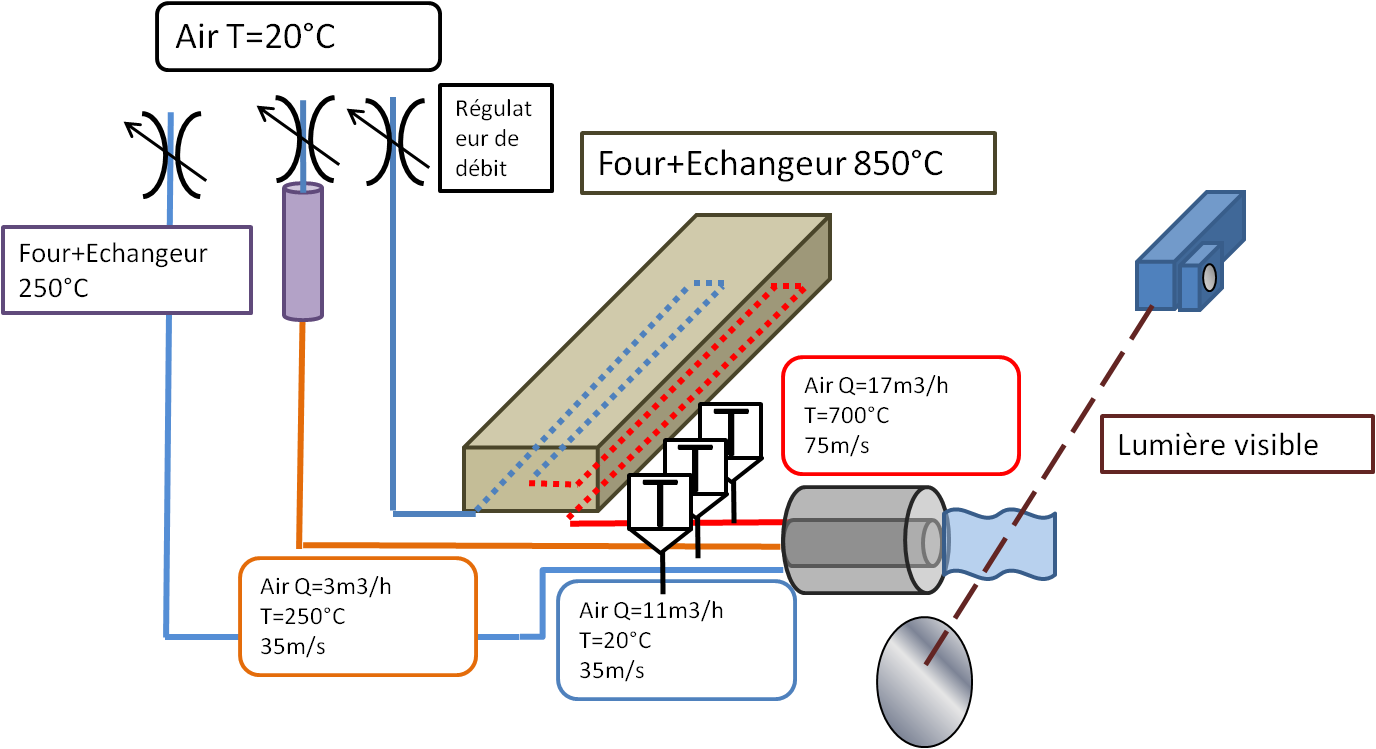
\includegraphics[width=0.8\textwidth]{fig/EPR_schema_installation.png}
  \caption{Schema de l'installation}
 \label{schema_installation}
\end{figure}

\begin{figure}[!h]
  \centering
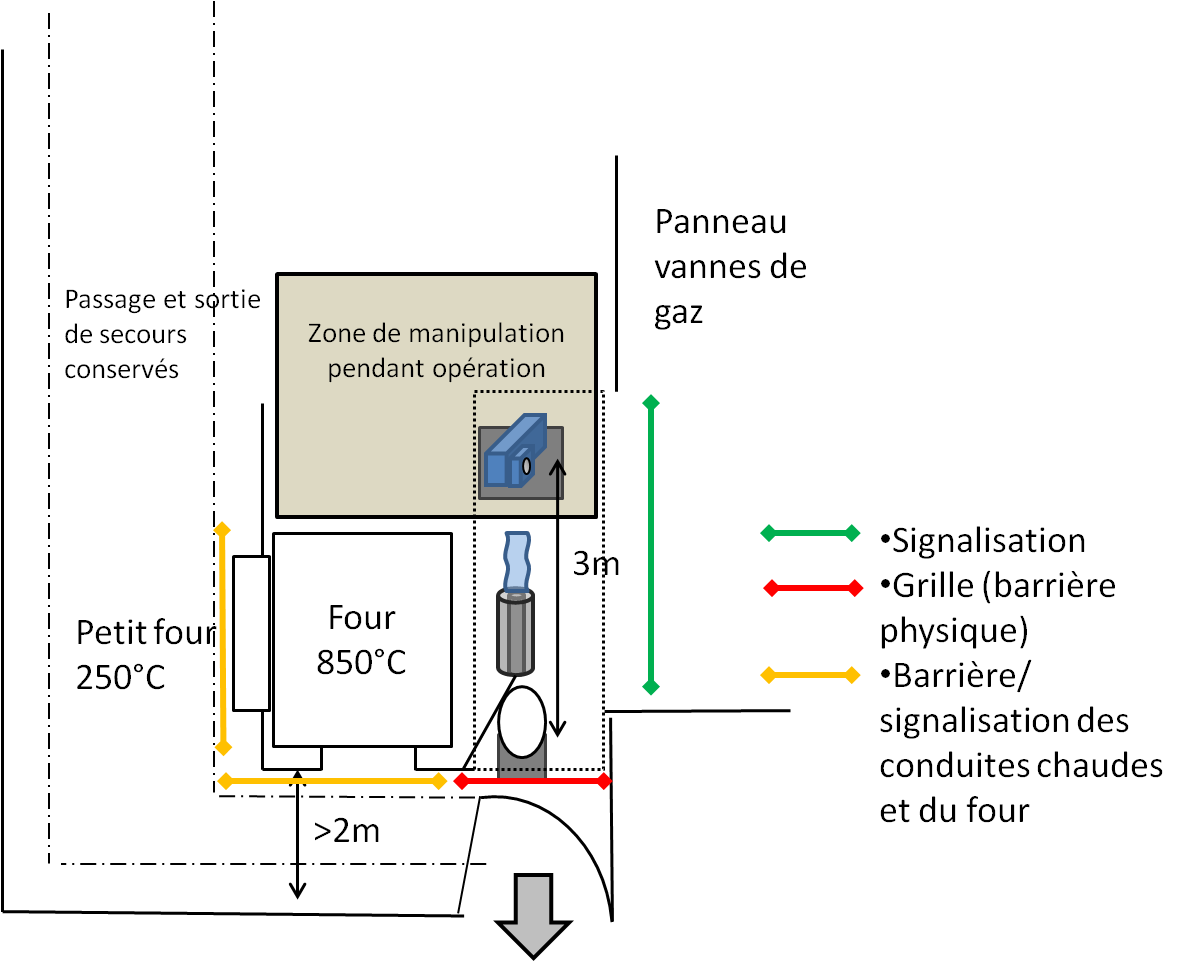
\includegraphics[width=0.8\textwidth]{fig/EPR_plan_de_travail.png}
  \caption{Plan de travail}
 \label{plan_travail}
\end{figure}
\newpage
\section{Plan de la manipulation}
\begin{enumerate}
\item Préparation
\begin{enumerate}
\item Disposition du matériel et raccordement à froid des trois arrivées d’air
\item Vérification de l'étanchéité
\item Réchauffeur placé dans le four
\item Four en position « pseudo-fermée » (25mm d’espace encore ouvert avant la butée)
\item Calorifugeage du four et des conduites d’air chaud
\item Calibration et focus du système optique sans écoulement
\item Changement de la consigne de sécurité du four pour que le four puisse démarrer en position « pseudo-fermée »
\item Balisage et pose des barrières de sécurité
\end{enumerate}
\item Mise en route
\begin{enumerate}
\item Chauffage des fours
\item Mise en écoulement de l’air
\item Asservissement de la température du four selon la consigne $T=600 ^\circ C$  pour l’air chaud
\end{enumerate}
\item Diagnostic/Mesures
\begin{enumerate}
\item Le diagnostic, les manipulations et ses éventuelles corrections optiques se font au minimum à une distance de deux mètres de l’écoulement
 \end{enumerate}
\item Fin de manipulation
\begin{enumerate}
\item Fermeture des débits d’air
\item Coupure des fours
\item Attente que le dispositif se refroidisse
 \end{enumerate}
\item Post Manipulation
\begin{enumerate}
\item Rétablir le seuil de sécurité d’origine du four (sécurité en butée : four fermé)
\item Etablir le procès verbal de fin d’opération
 \end{enumerate}
 \end{enumerate}
\section{Précautions particulières}
 On fera attention à :
 
 \begin{itemize}
\item Choisir des supports très stables pour le dispositif optique ainsi que le support du brûleur
\item Protéger la caméra rapide
\item L'écoulement d'air sera très bruyant, prévoir des protections
\end{itemize}




